\documentclass[aspectratio=169]{beamer}

%==============================================================================
% Geoptimaliseerde Presentatie Bachelorproef Arno Verhulst - Clean Version
%==============================================================================

\usetheme{hogent}
\usecolortheme{hgwhite}

\usepackage[dutch]{babel}  
\usepackage{csquotes}    
\usepackage{booktabs}          
\usepackage{multirow,multicol} 
\usepackage{eurosym}           
\usepackage{graphicx} 
\usepackage{tikz} % CRUCIAAL: Nodig voor de absolute positionering van het logo

%--- BIBLIOGRAFIE INSTELLINGEN (BibLaTeX + Biber) ---
\usepackage[style=apa, backend=biber]{biblatex}
\addbibresource{../bachproef/bachproef.bib}

%--- VISUELE OPMAAK INSTELLINGEN ---
\setbeamertemplate{footline}[frame number] % Strakke paginanummers rechtsonder
\setbeamertemplate{navigation symbols}{}   % Schakel navigatiesymbolen uit

% Metadata
\title{Optimalisatie van de Recovery Time Objective (RTO)}
\subtitle{in Active-Passive High Availability Clusters met Pacemaker en Corosync op RHEL-Nodes}
\author{\textbf{Arno Verhulst}}
\date{Academiejaar 2025-2026}

\begin{document}
    
    %---------- Slide 1: Aanpasbare Titelslide Met Logo ----------
    \begin{frame}
        % Zwevend logo rechtsonder plaatsen (stoort de tekstmarges niet)
        \begin{tikzpicture}[remember picture,overlay]
            \node[anchor=south east, xshift=-0.6cm, yshift=0.4cm] at (current page.south east) {
                
\includegraphics[height=0.8cm]{graphics/hogent_logo.eps}
            };
        \end{tikzpicture}
        
        \centering
        \vspace*{0.2cm} % Fijne marge aan de bovenkant
        
        % Hoofdtitel met de officiële Beamer-stijl van HOGENT
        {\usebeamerfont{title}\usebeamercolor[fg]{title}\Large\bfseries Optimalisatie van de Recovery Time Objective (RTO)} \\[0.2cm]
        
        % Subtitel in een iets compacter lettertype
        {\usebeamerfont{subtitle}\usebeamercolor[fg]{subtitle}\small in Active-Passive High Availability Clusters met Pacemaker en Corosync op RHEL-Nodes} \\[0.4cm]
        
        % Jouw naam prominent in het midden
        {\large \textbf{Arno Verhulst}} \\[0.4cm]
        
        % Opleidingsgegevens compact onder elkaar
        \footnotesize Professionele Bachelor Toegepaste Informatica \\
        Departement IT en Digitale Innovatie \\[0.4cm]
        
        % De promotors netjes uitgelijnd in een tabel
        \footnotesize
        \begin{tabular}{ll}
            \textbf{Promotor:} & Dhr. P. Beke \\
            \textbf{Co-promotor:} & Dhr. D. Allaert
        \end{tabular} \\[0.4cm]
        
        % Academiejaar als sluiting onderaan
        \small Academiejaar 2025-2026
    \end{frame}
    
    %---------- Slide 2: Inhoudsopgave ----------
    \begin{frame}
        \frametitle{Overzicht van de verdediging}
        \begin{center}
            \begin{minipage}{0.85\textwidth}
                \begin{block}{\textcolor{orange}{\textit{Agenda}}}
                    \begin{multicols}{2}
                        \tableofcontents
                    \end{multicols}
                \end{block}
            \end{minipage}
        \end{center}
    \end{frame}
    
    
    \section{1. Probleemstelling \& Context}
    
    %---------- Slide 3: De "Waarom" (Probleemschets) ----------
    \begin{frame}
        \frametitle{1. Probleemschets: De Kost van Downtime}
        \begin{columns}[c]
            \column{.65\textwidth}
            \begin{itemize}
                \item \textbf{Financiële Impact:} Ongeplande downtime kost grote ondernemingen al snel meer dan \textbf{\$300.000 per uur} \parencite{ITIC2024}.
                \item \textbf{Verborgen Kosten:} Schade aan de werknemersmoraal en acuut verlies van klantvertrouwen \parencite{Kollective2025}.
                \item \textbf{De Cloud Gap:} Standaard enterprise-instellingen schieten tekort binnen een software-defined cloudnetwerk \parencite{Microsoft2026}).
            \end{itemize}
            
            \column{.35\textwidth}
            \begin{alertblock}{RTO Baseline}
                Bij een harde node-crash of netwerkisolatie faalt de failover standaard volledig ($\infty$ downtime).
            \end{alertblock}
        \end{columns}
    \end{frame}
    
    
    \section{2. Onderzoeksvragen}
    
    %---------- Slide 4: DE HOOFDVRAAG ----------
    \begin{frame}
        \frametitle{2. De Hoofdonderzoeksvraag}
        \vspace{0.5cm}
        \begin{alertblock}{Centraal Uitgangspunt van het Onderzoek}
            \large\centering\itshape
            "Hoe kan een betaalbare Active-Passive High Availability webomgeving, bestaande uit Pacemaker en Corosync op RHEL-compatibele nodes, geoptimaliseerd worden om de Recovery Time Objective (RTO) van de webapplicatie bij serveruitval te minimaliseren?"
        \end{alertblock}
    \end{frame}
    
    %---------- Slide 5: DEELVRAGEN PROBLEEMDOMEIN ----------
    \begin{frame}
        \frametitle{2. Deelvragen: Probleemdomein}
        \begin{block}{Analyse van de Clusterstack}
            \begin{enumerate}
                \item \small Wat zijn de specifieke functies van Pacemaker, Corosync en STONITH (fencing) binnen de gekozen HA-architectuur, en hoe werken deze drie componenten samen om een consensus over de status van de webdienst te bereiken?
                \item \small Welke Pacemaker-configuratieparameters en constraints (zoals opstartinterval, resource-stickiness en timeoutwaarden) beïnvloeden het meest direct de snelheid van de failover en daarmee de RTO?
                \item \small Welke vereisten en risico's zijn cruciaal bij het gebruik van een virtueel IP-adres voor de webdienst in een Active-Passive cluster, en hoe beheert Pacemaker de migratie van dit virtuele IP om zero downtime bij failover te benaderen?
            \end{enumerate}
        \end{block}
    \end{frame}
    
    %---------- Slide 6: DEELVRAGEN OPLOSSINGSDOMEIN ----------
    \begin{frame}
        \frametitle{2. Deelvragen: Oplossingsdomein}
        \begin{block}{Implementatie, Validatie \& Kwantificering}
            \begin{enumerate}
                \item[4.] \small Hoe kan een robuust en betaalbaar Power Fencing-mechanisme (STONITH) -- cruciaal voor het garanderen van data-integriteit -- effectief geïmplementeerd en getest worden met behulp van een geschikte fence agent om 'split-brain'-scenario's betrouwbaar te voorkomen?
                \item[5.] \small Wat is de gemeten gemiddelde Recovery Time Objective (RTO) van de webdienst, gesimuleerd voor ten minste drie verschillende uitvalscenario's (bijvoorbeeld een harde nodecrash, een service crash, en netwerkisolatie)?
                \item[6.] \small Hoe kan de initiële Pacemaker-configuratie, op basis van de theoretisch geïdentificeerde parameters, stapsgewijs geoptimaliseerd worden om de RTO tot het laagst mogelijke niveau te reduceren, en wat is de impact van deze optimalisatie op de normale performantie van de webdienst?
            \end{enumerate}
        \end{block}
    \end{frame}
    
    
    \section{3. Stand van Zaken}
    
    %---------- Slide 7: Cloud Architectuur ----------
    \begin{frame}
        \frametitle{3. Stand van Zaken: Cloud Architectuur}
        \begin{columns}[c]
            \column{.5\textwidth}
            \begin{block}{Core Framework}
                \begin{itemize}
                    \item \textbf{Corosync:} Lidmaatschapsservice en heartbeat-monitoring via kronosnet \parencite{RedHat}.
                    \item \textbf{Pacemaker:} Cluster Resource Manager die via XML resources verdeelt \parencite{ClusterLabs}.
                    \item \textbf{STONITH:} Fysieke node-fencing voorkomt split-brain en data-corruptie \parencite{Luca2024}.
                \end{itemize}
            \end{block}
            
            \column{.5\textwidth}
            \centering
            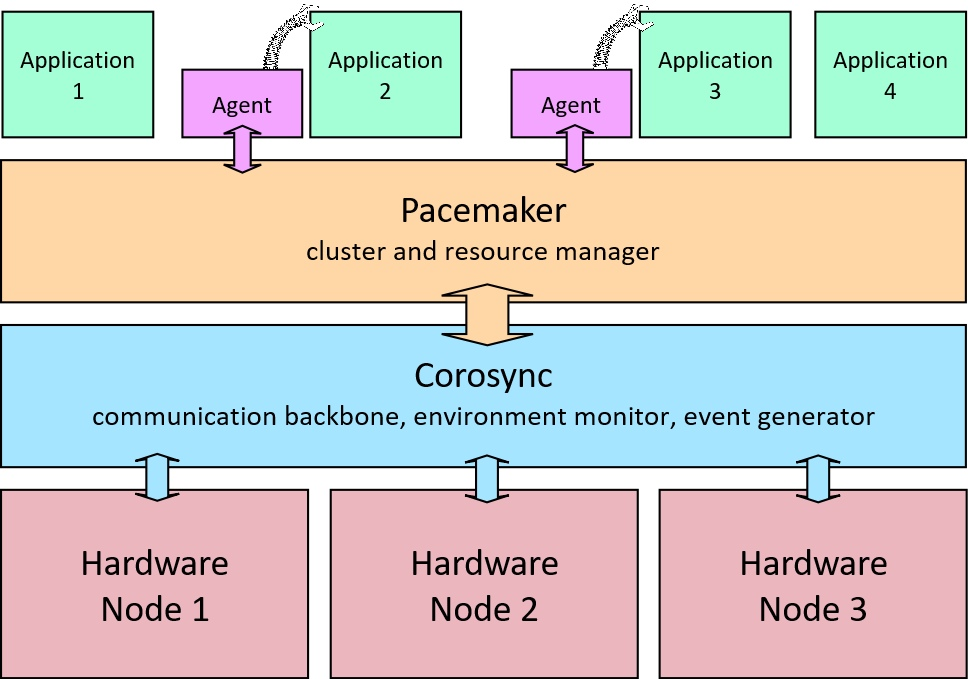
\includegraphics[width=\textwidth, height=0.45\textheight, keepaspectratio]{graphics/pacemaker}
            
            \vspace{0.15cm}
            \scriptsize 
            \textbf{Figuur 2.2:} De architecturale gelaagdheid van de clusterstack, met Corosync als fundament voor de communicatie tussen de hardware nodes \parencite{John2017}.
        \end{columns}
    \end{frame}
    
    
    \section{4. Methodologie}
    
    %---------- Slide 8: De 4 Fasen ----------
    \begin{frame}
        \frametitle{4. Methodologie: Experimentele Aanpak}
        \begin{columns}[c]
            \column{.45\textwidth}
            \centering
            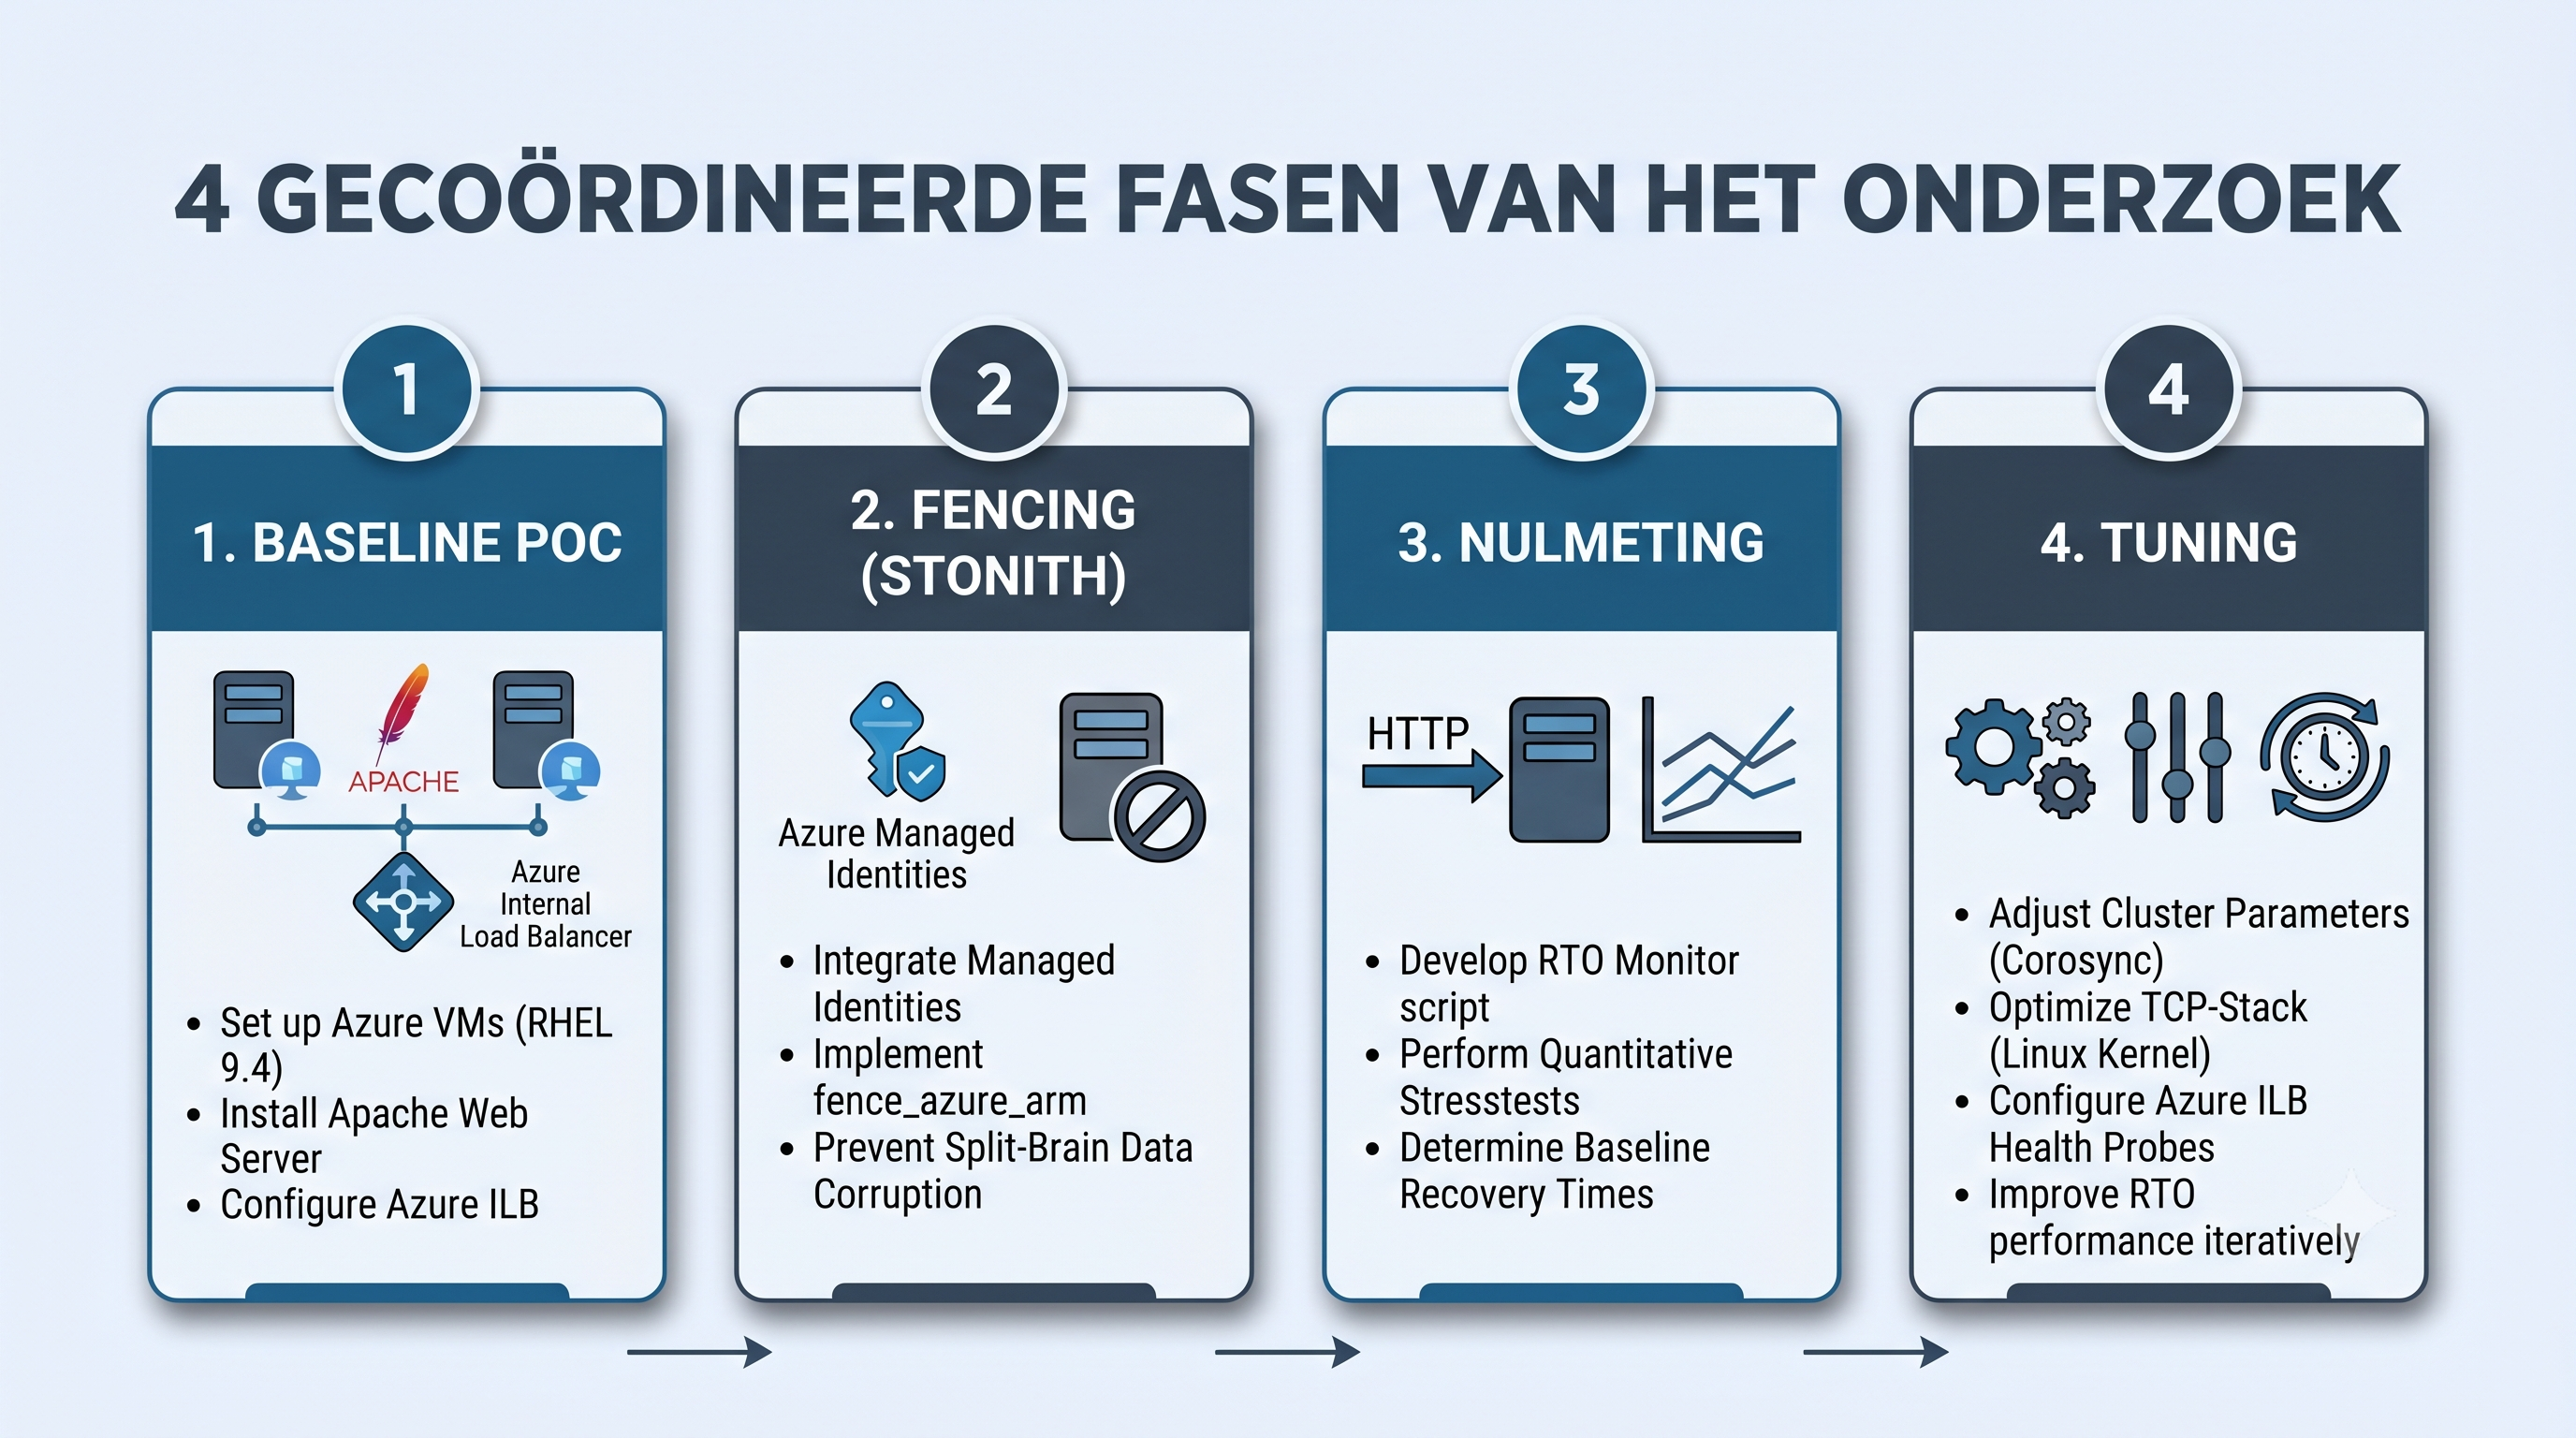
\includegraphics[width=\textwidth, height=0.45\textheight, keepaspectratio]{graphics/methodologie}
            
            \vspace{0.15cm}
            \scriptsize 
            \textbf{Figuur 4.1:} Visuele weergave van het onderzoeksproces \parencite{Gemini2026}.
            
            \column{.55\textwidth}
            \begin{itemize}
                \item \textbf{Fase 1 \& 2: PoC Setup:} VM provisioning op Azure (oXya-infra) en implementatie van \textbf{Managed Identities} voor STONITH (Stone, 2025).
                \item \textbf{Fase 3: Kwantitatieve Nulmeting:} Ontwikkeling van \texttt{rto\_monitor.sh} voor HTTP-polling elke 100ms.
                \item \textbf{Fase 4: Parameter-tuning:} Gecoördineerde tuning op cluster-, kernel- en cloud-netwerklaag.
            \end{itemize}
        \end{columns}
    \end{frame}
    
    
    \section{5. Proof of Concept}
    
    %---------- Slide 9: Parameter Tabel ----------
    \begin{frame}
        \frametitle{5. Gecoördineerde Parameter-Tuning}
        \begin{table}
            \centering
            \resizebox{0.95\textwidth}{!}{%
                \begin{tabular}{llll}
                    \toprule
                    \textbf{Niveau} & \textbf{Parameter} & \textbf{Baseline} & \textbf{Geoptimaliseerd} \\
                    \midrule
                    \textbf{Corosync Totem} & \texttt{token} & 3000ms & \textbf{500ms} \\
                    & \texttt{consensus} & 3600ms & \textbf{600ms} \\
                    \midrule
                    \textbf{Pacemaker Agent} & \texttt{monitor interval} & 60s & \textbf{2s} \\
                    & \texttt{resource-stickiness} & 1 & \textbf{100} \\
                    \midrule
                    \textbf{Linux Kernel}   & \texttt{tcp\_retries2} & 15 ($\approx$15m) & \textbf{5} (Pracucci, 2018) \\
                    \midrule
                    \textbf{Azure Netwerk}  & Floating IP (DSR) & Disabled & \textbf{Enabled} \\
                    & Health Probe Interval & 5s & \textbf{5s (Threshold 2)} \\
                    \bottomrule
                \end{tabular}%
            }
        \end{table}
    \end{frame}
    
    %---------- Slide 10: Gelaagde Architectuur ----------
    \begin{frame}
        \frametitle{5. Proof of Concept: Gelaagde Architectuur}
        \begin{center}
            
\includegraphics[width=0.65\textwidth, height=0.45\textheight, keepaspectratio]{netwerkschema}
            
            \vspace{0.15cm}
            \scriptsize 
            \textbf{Figuur 4.1:} Uiteindelijk netwerkschema van de geoptimaliseerde Active-Passive HA-omgeving binnen de Azure Resource Group \parencite{Gemini2026}.
        \end{center}
    \end{frame}
    
    
    \section{6. Resultaten \& Conclusie}
    
    %---------- Slide 11: De Resultaten ----------
    \begin{frame}
        \frametitle{6. Resultaten: Kwantitatieve Vergelijking}
        \begin{center}
            \begin{minipage}{0.85\textwidth}
                \begin{table}
                    \centering
                    \resizebox{\textwidth}{!}{% Dit dwingt de tabel binnen de breedte van de minipage
                        \begin{tabular}{lrrr}
                            \toprule
                            \textbf{Uitvalscenario} & \textbf{RTO Baseline} & \textbf{RTO Geoptimaliseerd} & \textbf{Winst} \\
                            \midrule
                            1. Service-level failure & 10,80s & \textbf{1,33s} & 87,7\% \\
                            2. Netwerkisolatie (Split-brain) & $\infty$ (Faal) & \textbf{3,37s} & \textbf{$>$99\%} \\
                            3. Node-level crash (Harde crash) & $\infty$ (Faal) & \textbf{2,03s} & \textbf{$>$99\%} \\
                            \bottomrule
                        \end{tabular}%
                    }
                \end{table}
                
                \begin{alertblock}{Overtuigend Resultaat}
                    Door gecoördineerde tuning over de hele stack zakt de RTO met \textbf{meer dan 90\%}. Een abrupte node-crash herstelt sneller dan een graceful shutdown wegens het direct skippen van time-outs.
                \end{alertblock}
            \end{minipage}
        \end{center}
    \end{frame}
    
    %---------- Slide 12: Conclusie Matrix ----------
    \begin{frame}
        \frametitle{6. Kritische Evaluatie \& Conclusie}
        \begin{table}
            \centering
            \resizebox{0.95\textwidth}{!}{%
                \begin{tabular}{lll}
                    \toprule
                    \textbf{Onderzocht Aspect} & \textbf{Gemaakte Keuze / Resultaat} & \textbf{Impact \& Risico (Trade-off)} \\
                    \midrule
                    \textbf{Cluster Stack Tuning} & Token gereduceerd naar 500ms & \alert{Risico op 'False Positives'} bij cloud-netwerk jitter. \\
                    \textbf{Cloud Netwerk Integratie} & Floating IP / DSR geactiveerd & Cruciale randvoorwaarde voor Azure ILB routering. \\
                    \textbf{Split-Brain Preventie} & Azure Power Fencing via API & Waterdichte data-integriteit zonder shared storage. \\
                    \textbf{Beveiliging} & Gebruik van Managed Identities & Geen hardcoded credentials binnen de cluster-stack. \\
                    \bottomrule
                \end{tabular}%
            }
        \end{table}
        \centering
        \vspace{0.1cm}
        \small\textit{Conclusie: Een RTO van enkele seconden is stabiel haalbaar, mits cloud-specifieke netwerkarchitecturen gerespecteerd worden.}
    \end{frame}
    
    %---------- Slide 13: Q&A Sluiting Met Logo ----------
    \begin{frame}
        % Zwevend HOGENT-logo rechtsonder geplaatst op de afsluitende slide
        \begin{tikzpicture}[remember picture,overlay]
            \node[anchor=south east, xshift=-0.6cm, yshift=0.4cm] at (current page.south east) {
                
\includegraphics[height=0.8cm]{graphics/hogent_logo.eps}
            };
        \end{tikzpicture}
        
        \centering
        \huge \textbf{Bedankt voor uw aandacht.} \\
        \bigskip
        \vspace{0.8cm}
        \begin{center}
            \small \textbf{Arno Verhulst} -- \texttt{arno.verhulst@student.hogent.be} \\
            \small Git Repository: \href{https://github.com/vharno1612/bachelorproef-2526-vharno1612.git}{\color{blue}\underline{github.com/vharno1612/bachelorproef-2526-vharno1612}}
        \end{center}
    \end{frame}
    
    %---------- Slide 14: Dynamische Referentielijst ----------
    \section{7. Referenties}
    \begin{frame}[allowframebreaks]
        \frametitle{Referenties}
        \printbibliography
    \end{frame}
    
\end{document}